
\documentclass[
  ngerman
  ,12pt
  ,pdftex
]{article}

\usepackage{graphicx}
\usepackage{amsmath}
\usepackage{amssymb}
\usepackage{listings}
\usepackage[ngerman]{babel}
\usepackage[utf8]{inputenc}
\usepackage[T1]{fontenc}
\usepackage{alltt}

\hyphenation{Differential-gleichung}
\hyphenation{Über-tragungs-ope-ra-tors}
\hyphenation{E/A-Differential-gleichung}

\begin{document}
\section{Fragen}
\begin{enumerate}
  \item Lösung des Shift/Reduce Konflikt. Was steht auf dem Keller? Was ist das nächste Zeichen?
  \item Wie funktioniert der Keller im Bezug auf die Elimation der linksrekursion? Script Seite 174
  \item Wie geh ich mit Mehrdeutigkeit um im Shift Reduce Kontext?
  
  \item Nicht-deterministischer Übergang?
  \item Teilkonstruktion Mengen?
  \item Wie löse ich den Reduce/Reduce Konflikt?
  \item Wie geh ich bei Lark vor?
  \item Wie gehe ich mit dem Ast um?
  \item Wie wird Parser/rex umgesetzt?
  \begin{itemize}
    \item []  Ich antworte ihr auf die Frage  
  \end{itemize}
\end{enumerate}
\section{Aufgaben}
Auf Seite 7 im Script sind die Übungsaufgaben verzeichnet\\
Laut den Alt-Klausuren
\begin{itemize}
  \item Strukturierung von einem Übersetzer
  \item Fragen zur Grammatik!!!
  \begin{itemize}
    \item []  rechts links regulär definition
    \item []  Pumping Lemma (Siehe Inkodo Fragen)
    \item []  Kontextfrei/Kontextsensitive
  \end{itemize}
  \item Chomsky-Hierarchie
  \begin{itemize}
    \item []  Arten von Grammatik 0 bis 3
  \end{itemize}
  \item Lark+Ast oder Rex
  \item Lark-Spezifikation
  \item Top-Down-Parser/Rekursiver Abstiegs-Parser
  \item Abstrakter Syntaxbaum
  \begin{itemize}
    \item Grammatik 
    \item Automat
    \item Ableitung
  \end{itemize}
\end{itemize}
\subsection{Laut Vollmer}
\begin{itemize}
  \item Scanner
  \item Baum
  \item rekursiver Abstiegsparser (ist ein LL-Automat)
  \item Makefile nicht
  \item LL-Automat Mengen schneiden
  \item Lark-Spezifikationen
  \item Rex
  \item Insert Rules in der Reihenfolge da sonst First-Rule-Match
  \item Abstrakter Syntaxbaum
  \item Parser (ist ein LR-Automat) -Spezifikation
  \item Algorithmus: AST-Aufbau Button-Up
  \item Attibut Grammatik 
  \item Funktionale Spezifikation einer Attributberechnung (Baum gegeben)
\end{itemize}
Andere Aufgaben
\begin{itemize}
  \item Quiz File
  \item Teilmengenkonstruktion NEA in DEA Automat zeichnen
  \item 
\end{itemize}
\section{LL-Eigenschaften}
Seite 166 im Script stehen die Eigenschaften \\
Wie andere Grammatik transformiert findet man im Script auf Seite 169
Eine Grammatik kann nicht die LL-Eigenschaften erfüllen wenn sie linksrekursion bzw. linksgleiche Produktionen enthält (Was sind Produktionen?)
Allgemeine Elimination von linksrekursion auf Seite 171 im Script
\begin{align*}
    A::= A \alpha \\
    \Longrightarrow \\
    A::= \beta A' \\
    A'::=\alpha A' | \epsilon
\end{align*}

Definition (Linksfaktorisierung). Problem $FIRST(..FOLLOW(..))$ nicht disjunkt:
\begin{align*}
  A::=\alpha \beta_1  |  \alpha \beta_2 \\
  \Longrightarrow\\
  A::= \alpha A'\\
  A'::= \beta_1  |  \beta_2
\end{align*}
$FF_1 = FIRST(T E' FOLLOW(E))={i*}$ das in den geschweiften Klammern ist das $First(T)$ wenn $\epsilon$ nicht in der First-Menge ist. 
Falls doch ist es das $First$ vom nächssten nicht Terminal. 
Falls alle ein $\epsilon$ in ihrer First\_Menge haben ist es das $Follow(E')$.\\
\\

\subsection{LL-Bedingungen \label{ref}}
Die Grammatik erfüllt die LL-Bedingungen wenn die gleichen Follows in den First-Follow-Mengen einen unterschiedlichen Inhalt haben.
\begin{align*}
  FF_1 = FIRST(T E' FOLLOW(E))={i*}\\
  FF_2 = FIRST(\epsilon FOLLOW(E))={\#}
\end{align*}



\subsection{LL-Automaten}
Seite 177 findet man die LL-Automaten \\
\begin{itemize}
  \item Der LL-Automat erzeugt eine Linksableitung des Eingabewortes
  \item Erfüllt $G$ die LL-Bedingungen, dann kann ein deterministischer Automat konstruiert werden.
\end{itemize}

\begin{enumerate}
  \item Transfomieren Sie die Grammatik, so dass die Grammatik die LL(1) Bedingung erfüllt
  \item Erstellen Sie den nichtdeterministischen LL(1)-Automaten für diese Grammatik
  \item Erstellen Sie hieraus den deterministischen LL(1)-Automaten\\ (nun ja er ist nicht ganz deterministisch, da die Produktionen eines Nichtterminals die LL(1) Bedingung nicht erfüllt, erstellen Sie den Automaten trotzdem!)\\
  Markieren Sie die nichtdeterministischen Automatenregeln.
  \item Akzeptieren Sie mit diesem Automaten das "Programm" i + i[i+i]
\end{enumerate}
Beispiel Aufgabe auf Seite 179 im Script\\
\begin{itemize}
  \item Grammatik linksrekursion rausbekommen
  \item First-Follow-Menge berechnen 
  \item LL1 Eigenschaften herausfinden
  \item Automat
  \item Automat mit First-Follow
\end{itemize}
Die Regel schreib man einfach umgekehrt zur Grammatik.
\begin{align*}
  E' ::= +TE'\\
  E'qt\longrightarrow E'T+
\end{align*}


\section{LR-Automaten}

\begin{center}
  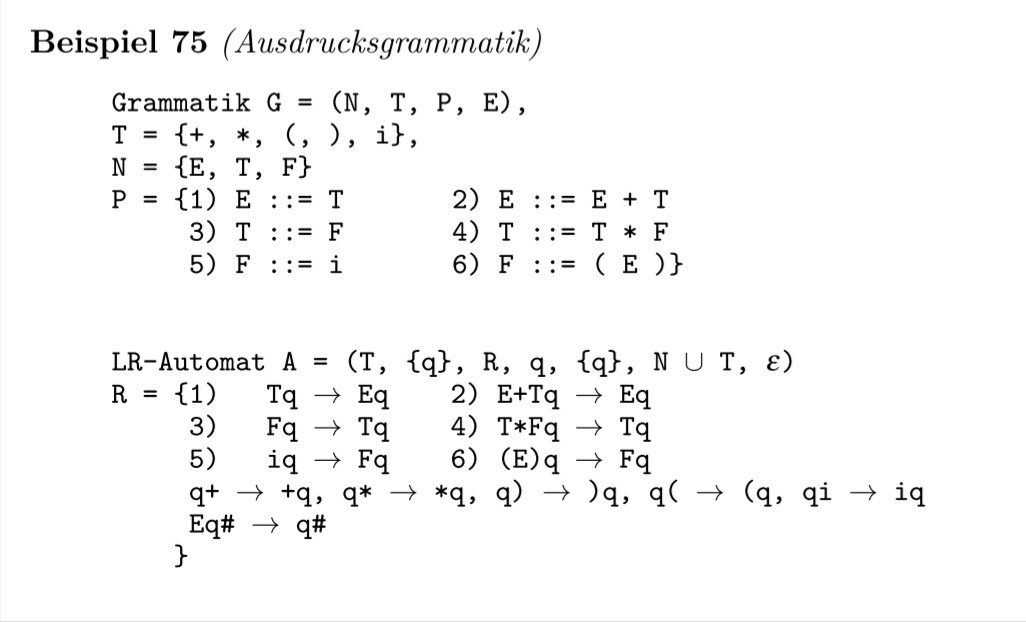
\includegraphics[height=7cm]{image/Screenshot 2022-12-10 170319.jpg}
\end{center}
\begin{center}
  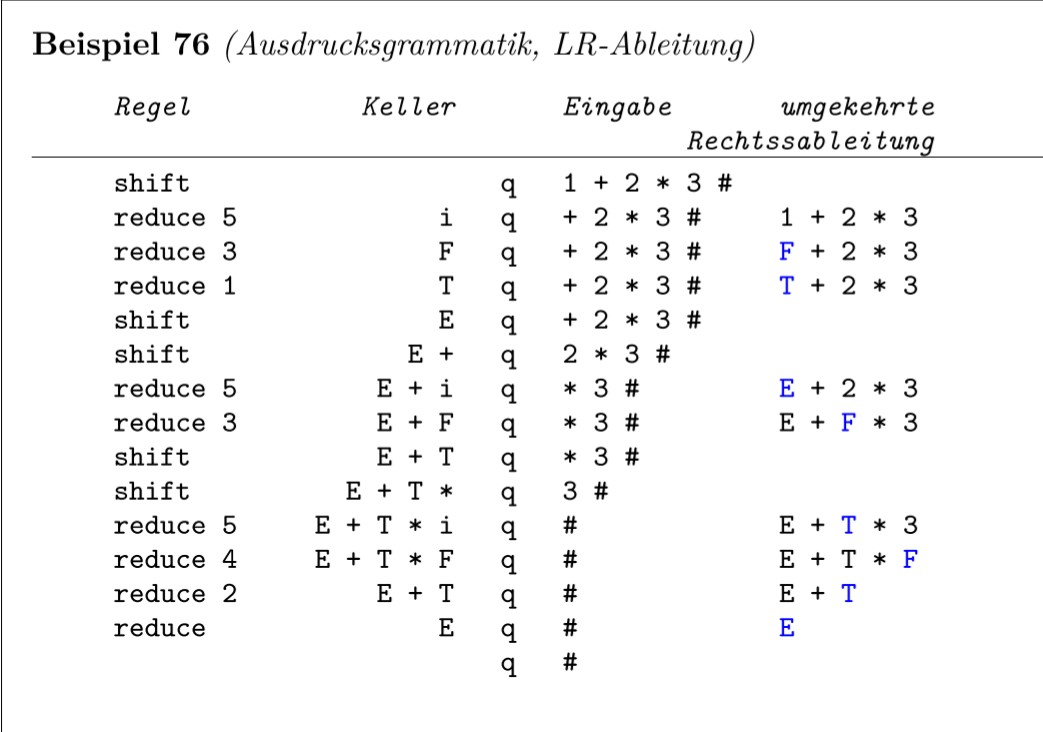
\includegraphics[height=7.5cm]{image/Screenshot 2022-12-10 170336.jpg}
\end{center}
\subsection{Konflikte}
\subsubsection*{Shift/Reduce}
Mehrdeutigkeit wird unterbunden in dem bevorzugt gesschiftet wird. $\Longrightarrow$ Lösung Dangeling-Else Problem.
Nicht immer shiften Operatorvorrang (Skript Seite 198f)
\subsubsection*{Reduce/Reduce}
Macht es einen Unterschied?\\
Wenn nicht eine Regel wegschmeisen 

\section{Struktur vom Compiler}
\begin{enumerate}
  \item Wozu kann ein Übersetzerbenutzt werden?
  \begin{itemize}
    \item [] Erzeugen von Maschinencode 
    \item [] Programmanalyse und das Füllen einer Datenbank mit Informationen über das Programm
    \item [] Programmtransformation in eine andere Programmiersprache
  \end{itemize}
  \item Wie ist ein Übersetzer strukturiert? Beschreiben Sie \textbf{kurz} die Aufgaben und Ergebnisse der einzelen Phasen!
  \begin{itemize}
    \item []1. Lexikalische Analyse, 2.syntaktische Analyse, 3. Transformation(nicht ausreichend)
  \end{itemize}
  \item Welche Rolle spielt die Grammatik in einer Sprache?
  \begin{itemize}
    \item [a]Eine Grammatik dient zur Spezifikation der Programmiersprachr für den Benutzer der Sprache, damit dieser weiß, wie ein korrektes Programm geschriebenwerden kann(ANleitung zum Generieren eines Satzes der Sprache).
    \item [b]Eine Grammatik dient zur Spezifikation des Übersetzters für diese Programmiersprache(Anleitung zur Konstruktion eines Akzeptors für diese Sprache).
  \end{itemize}
\end{enumerate}
\section{Fragen zur Grammatik}
\begin{enumerate}
  \item Geben sie die Definition einer regulären Grammatik an.
  \begin{itemize}
    \item [] $G=(N,T,P,Z)$, Nichtterminale(z.B. E,T,D die Dinge mit denen man die Regeln macht), Terminale = Symbole(z.B. +,-,*),Produktion (Regel), Startsymbol
  \end{itemize}
  \item Geben sie die Definition des Begriffes der von einer Grammatik erzeugten Sprache an.
  \begin{align*}
    L=\{w\in T* | Z \Longrightarrow*w\}
  \end{align*}
  \begin{itemize}
    \item Kein Plan was das heißen soll steht auch auf Seite 71 im Script
  \end{itemize}
  \item Geben Sie die Definition eines endlichen Automaten an.
  \item Geben sie die Definition der von diesem Automaten akzeptierten Sprache an.(Welche Art von Sprachen wird vom Automat akzeptiert)
  \item Was ist der Zusammenhang zwischen einem endlichen Automaten A, der die von G erzeugte Sprache akzeptiert.
  \begin{itemize}
    \item Zu jeder regulären Grammatik G gibt es einen endlichen Automaten A, der die von G erzeugte Sprache akzeptiert(Gibt einen Beweis aber kein bock den hinzuschreiben oder zu lernen)

  \end{itemize}
  \item Was ist der Zusammenhang zwischen deterministischen und nichtdeterministischen endlichen Automaten?
  \begin{itemize}
    \item Zu jedem nichtdeterministischen endlichen Automaten gibt es einen deterministischen endlichen Automaten, der die gleiche Sprache akzeptiert.
  \end{itemize}
  \item  Es wird eine Sprache beschrieben an dieser sollen folgende Aufgaben durch geführt werden
  \begin{itemize}
    \item [a] Die rechts reguläre Grammatik soll für die Sprache angegeben werden.
    \item [b] Für die Grammatik soll der Endliche Automat angegeben werden. (eigentlich dann mit Shift und Reduce)
    \item [c] Stellen sie ihren Automaten graphisch dar. Kennzeichnen Sie Start- und Finalzustände.
    \item [d] Ist Ihr Automat deterministisch? Falls nein,kennzeichnen Sie nicht-deterministischen Übergänge.
  \end{itemize}
  \item Konstruieren Sie (mittels des aus der Vorlesung bekannten Verfahrens) den deterministischen
  endlichen Automaten, der die von Ihnen definierten C-Bezeichner akzeptiert. Zeichen Sie den resultierenden
  Automaten(Es ist die Teilmengen Konstruktion)
\end{enumerate}

\subsection{Chomsky-Hierarchie}
\begin{itemize}
  \item [] \textbf{Typ-0, rekursiv aufzählbar}
  \item [] \textbf{Typ-1, kontextsensitiv}
  \begin{itemize}
    \item [] $xAy::=xwy$
    \item [] Ist $Z \longrightarrow \epsilon$, dann darf $Z$ nicht auf der rechten Seite einer Regel vorkommen.
  \end{itemize}
  \item [] \textbf{Typ-2, kontextfrei}
  \begin{itemize}
    \item []$A \longrightarrow w$
    \item [] Keller TM
    \item [] Nichtterminal durch Wort ersetzen entweder rechts oder links regulär
  \end{itemize}
  \item [] \textbf{Typ-3, regulär}
  \begin{itemize}
    \item [] $A \longrightarrow a$ oder $A \longrightarrow \epsilon $
    \item [] Nichtterminal weder durch eine Folge an Zeichen ersetzt
    \item [] \textbf{rechts-regulär} $A \longrightarrow aB$
    \item [] \textbf{links-regulär} $A \longrightarrow Ba$
  \end{itemize}
\end{itemize}
\subsection{Pumping Lemma}
$a^nb^n$ ist das Kammagebirge ..(()).. ist nicht regulär und verletzt das Pumping Lemma\\
xabz\\
xababz \\
xaaabbbz das geht nicht deswegen nicht regulär
\subsection*{Lexikalische Analyse / Scanner-Generator: Rex}
\textbf{Eingabe}
\begin{itemize}
    
    \item [-] Quelltext = Folge (ASCII) Zeichen
\end{itemize}
\textbf{Ausgabe}
\begin{itemize}
    \item [-] Folge von Symbole
    \item [-] Attribute für Token
\end{itemize}
\textbf{Aufgaben}
\begin{itemize}
    \item [-] Zusammenfassung von (ASCII) Zeichen zu Token
    \item [-] Überlesen von Leerzeichen und Kommentaren
    \item [-] Konvertierung / Normalisierung
    \item [-] Berechnung der Token-Attribute
\end{itemize}
\textbf{Spezifikationsmethode}
\begin{itemize}
    \item [-] Reguläre Ausdrücke
    \item [-] Regeln zur Auflösung von Mehrdeutigkeiten???
    \item [-] Semantische Aktionen (C-Anweisungen)\\
\end{itemize}
In der Klausur sollen die Spezifikationen definiert werden. 
\begin{enumerate}
    \item Vordefinerte Regeln
    \item Benannte reguläre Ausdrücke
    \item Schlüsselwörter sind case-inte siehe Skript Seite 145
    \item Ganze Zahl oder Festkommazahl?
    \item Bezeichner oder Schlüsselwört?
    \item Kommentare Überlesen
    \item DEA: Und erkann doch zählen!
    \item String-Literale akzeptieren und transformieren
\end{enumerate}
\subsection{Benannte reguläre Ausdrücke}
Häufig benötigt man einen (komplexen) Ausdruck 
mehrfach in einer Scannerspezifikation, z. B. $\textbf{ \{ 0 -9 \} }$ oder $\textbf{\{a-zA-Z\_\}}$. 
Anstatt diese nun immer wieder in den Regeln zu notieren, kann man auch sogenannte benannte reguläre Ausdrücke benutzen.\\
Der Ausdruck wird in \textbf{DEFINE} definiert und in \textbf{Rule} wird die Benutzung definert.
%\input{inputs/BenanntereguläreAusdrücke.tex}
In der Klausur vllt bool
\subsection*{Pattern Matches-Regel}
\subsection*{Regel: First Rule Matches}
Gibt es mehrere regulären Ausdrücke in einer Scannerspezifikation, welche alle die aktuellen Zeichen $z_0z_1z_2 . . . z_n$ der Eingabe akzeptieren würden, wird
die Regel zur Akzeption ausgewählt, welche textuell zuerst in der Scannerspezifikation steht.


\subsection{Teilmengenkonsstruktion (Arbeitslistenalgorithmus)}
\begin{enumerate}
    \item Zeichne eine Tabelle(DEA, Zustände, NEA)
    \item Starte mit dem Startsymbol und führe einen neuen Zustand ein.
    \item Folge den Produktionen des Startzutands und erzeuge für die erreichbare Zustände durch ein Terminalsymbol im DEA, einen neuen Zustand.
    \item Wiederhole die Suche nach erreichbaren Zuständen für alle anderen Zustände des erzeugten DEAs, solange bis sich nichts mehr ändert
\end{enumerate}
\begin{center}
    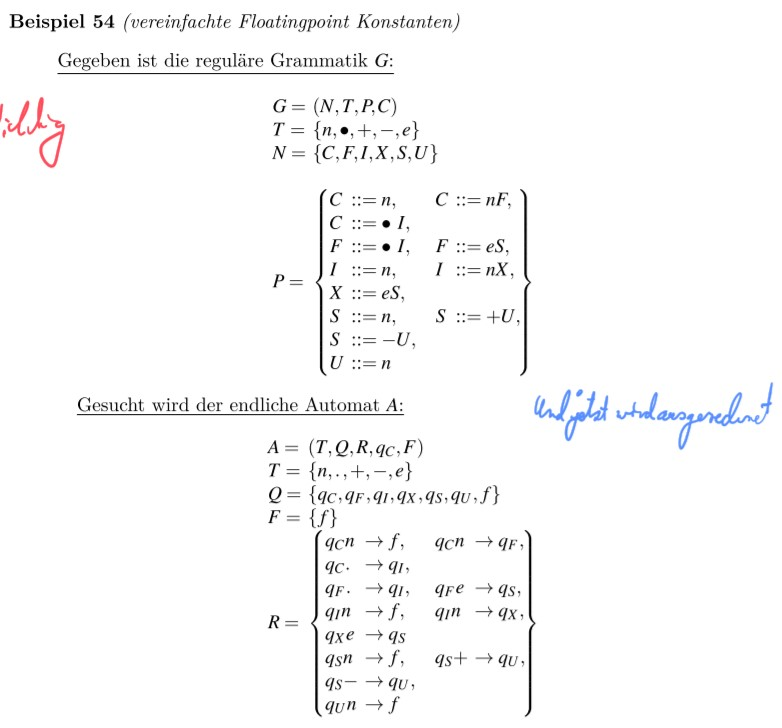
\includegraphics[height=7.5cm]{image/Tabelle_Teilmengen.jpg}
  \end{center}
\end{document}